\section{Evaluation}
\label{sec:evaluation}
This section presents our experiments with a case study of developing a software application for LEGO to evaluate the feasibility and usability of XSeparation.
The latter is implemented as an extension of the Papyrus modeling tool, which is based on Eclipse.
Architecture models in UML and XSeparation-generated C++ are synchronized.
Our XSeparation compiler supports POSIX systems, in which pthreads are used for executing concurrency in UML State Machines such as doActivity or infinite loop for event dispatching.
The usage of C++11 standard threads can be easily integrated in the future.
For incremental code generation in XSeparation, a model listener based on IncQuery is hooked to the modeling tool to detect model modifications.

The additional constructs added to C++ are engineered in a way that allows programmers to use facilities such as auto-completion of any C++ IDE to write interaction code between components or state machine descriptions.
It means that the programmers can stay within their familiar IDE and its facilities to effectively write code.
This is one of our advantages over other approaches which will be discussed in Section \ref{sec:relatedwork}. 
For example, Fig. \ref{fig:autocompletion} shows auto-completions for writing interaction codes for the examples in case using interface and data ports within Eclipse CDT ((a) and (b)) and Visual Studio ((c) and (d)).
Note that no additional tools need to be required for the auto-completions.

\begin{figure}
	\centering
	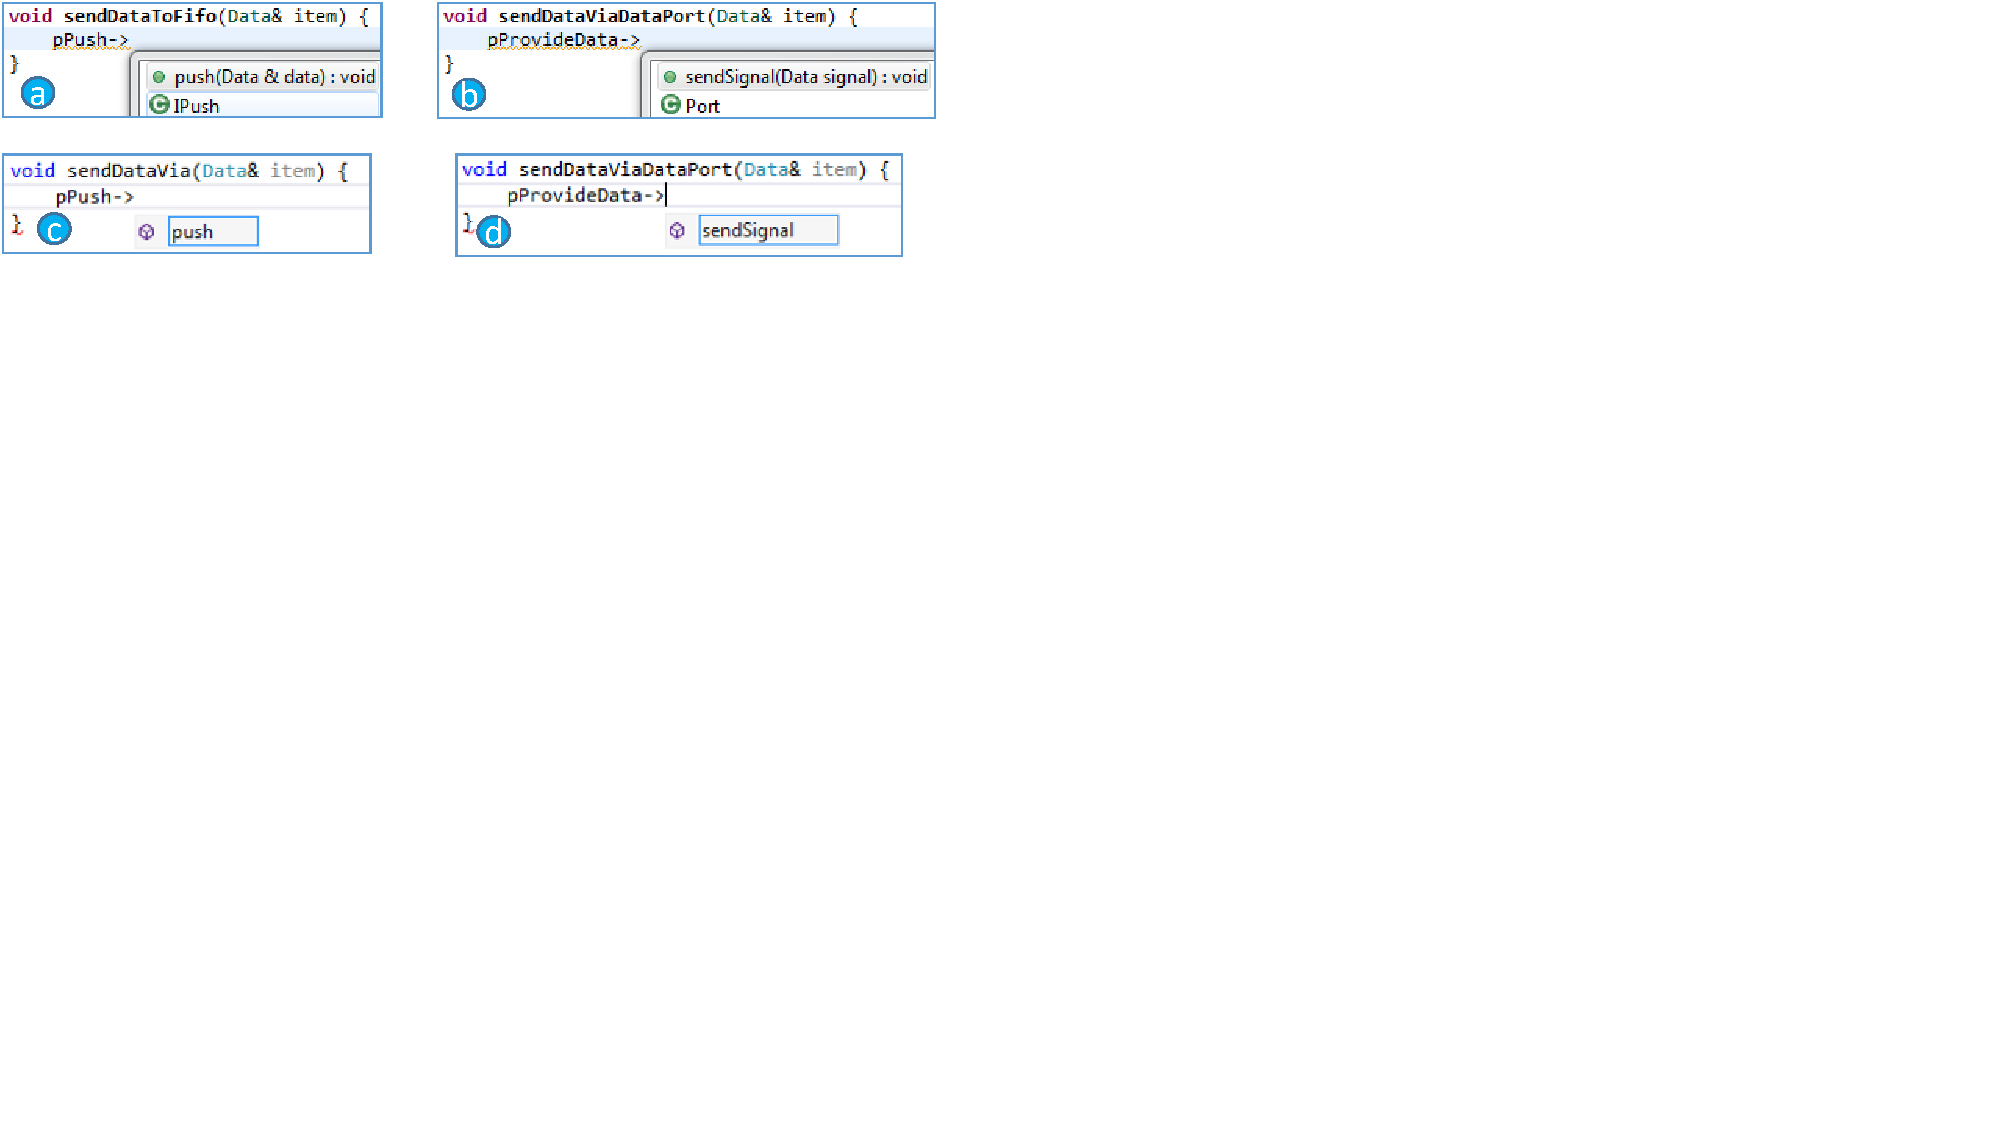
\includegraphics[clip, trim=0cm 14.6cm 17.7cm 0cm, width=\columnwidth]{figures/autocompletion.pdf}
	\caption{Auto-completions for XSeparation-generated code from the examples with interface and data ports: (a) and (b) in CDT and (c) and (d) in Visual Studio} 
	\label{fig:autocompletion}
\end{figure}

After implementation, we then developed a software application for LEGO in order to evaluate XSeparation through the tooling prototype.
The followings present the case study development for the applicability evaluation and a manual evaluation of the usability.
%\subsection{Implementation}

\subsection{Case study development}
Description of the application...

The case study was developed by a developer. She used the Papyrus Designer tool, which is component-based and model-driven development and features full C++ code generation.
UML models are used for the software and allow to embed fine-grained code as blocks of texts within a plain text editor.   

During the development, a software model is created.
However, the developer felt difficult, unfamiliar, and annoyed to write code with a limited editor.
She then refused to use that editor and programmed in CDT to be familiar and effective because of CDT facilities such as C++ syntax highlights and auto-completion.
She then copied the code from CDT to the model and regenerated the code.
Although the latter was compiled, the developer felt inefficient, prone-to-error, and lack comprehension of the architecture information generated from the model during code writing and copying.

Given the above issues, the developer wants to try a synchronization approach, which at least can automatically synchronize modifications in fine-grained code to the model.


%\subsection{Evaluations of Incremental code generation and reverse engineering in XSeparation}

\subsection{Usability evaluation}
To evaluate the usability of XSeparation, several questions are used for asking developers for how effective XSeparation is when compared to full code generation approaches using fine-grained code directly embedded within models.

\paragraph{Is model-code synchronization in XSeparation better than full code generation with fine-grained code within models in general?}

\paragraph{Is modifying architecture at the code level more effective than at the model level?}

\paragraph{Is modifying fine-grained code at the code level better than code embedded within models for full code generation?}

\paragraph{Is concurrent development using XSeparation effective?}

